\chapter{图中的路径 (Paths in graphs)}

\section{距离 (Distances)}

深度优先搜索能够轻而易举地找出从指定起点出发所能到达的图的所有顶点。它还能在搜索树中给出到达这些顶点的显式路径（图 4.1）。然而，这些路径未必是尽可能最经济（最短）的路径。在图 4.1 中，从 $S$ 出发只需经过 1 条边即可到达顶点 $C$，而 DFS 树给出的路径长度却为 3。本章的主题就是寻找图中\textbf{最短路径 (shortest paths)} 的算法。

路径长度使我们能够定量地探讨图中不同顶点之间的分离程度：
\begin{center}
    \textbf{两个节点之间的距离 (distance)，是指连接它们的最短路径的长度。}
\end{center}
为了直观体会这一概念，设想图的一个物理实体模型：每个顶点用一个小球表示，每条边用一段固定长度的细绳表示。如果你将代表起点 $s$ 的小球提得足够高，随着它一同被悬空提起的其他小球，恰恰就是从 $s$ 可达的顶点集合。要测量它们到 $s$ 的距离，只需测量它们悬挂在 $s$ 下方的垂直距离即可。

\begin{figure}[htbp]
\centering
\begin{tikzpicture}[scale=0.85, auto, >=latex]
    % (a) 简单图
    \begin{scope}[shift={(0,0)}]
        \node[circle,draw,fill=blue!15,inner sep=2pt] (S) at (0,1) {S};
        \node[circle,draw,inner sep=2pt] (A) at (1.5,2) {A};
        \node[circle,draw,inner sep=2pt] (B) at (3,2) {B};
        \node[circle,draw,inner sep=2pt] (C) at (1.5,0) {C};
        \node[circle,draw,inner sep=2pt] (D) at (3,0) {D};
        \node[circle,draw,inner sep=2pt] (E) at (0,-0.5) {E};

        \draw[thick] (S)--(A) (A)--(B) (B)--(D) (D)--(C) (C)--(S) (C)--(E) (D)--(E);
        \node at (1.5,-1.2) {(a) 简单图};
    \end{scope}

    % (b) DFS 树
    \begin{scope}[shift={(5.5,0)}]
        \node[circle,draw,fill=blue!15,inner sep=2pt] (tS) at (0,2) {S};
        \node[circle,draw,inner sep=2pt] (tA) at (1,2) {A};
        \node[circle,draw,inner sep=2pt] (tB) at (2,2) {B};
        \node[circle,draw,inner sep=2pt] (tD) at (2,1) {D};
        \node[circle,draw,inner sep=2pt] (tE) at (1,1) {E};
        \node[circle,draw,inner sep=2pt] (tC) at (0,1) {C};

        \draw[thick,->] (tS)--(tA); \draw[thick,->] (tA)--(tB);
        \draw[thick,->] (tB)--(tD); \draw[thick,->] (tD)--(tE);
        \draw[thick,->] (tE)--(tC);
        \node at (1,-1.2) {(b) DFS 树 (S 到 C 长度为 5)};
    \end{scope}
\end{tikzpicture}
\caption{简单图与其深度优先搜索树对比}
\label{fig:path_intro}
\end{figure}

在图 4.2 的物理模型中，当 $S$ 被提起时，沿最短路径的绳子被紧紧拉直（绷紧）。而不在任何最短路径上的边（例如边 $(D, E)$）则保持松弛状态。

\section{广度优先搜索 (Breadth-first search)}

提起节点 $s$ 将整张图自然地划分为了若干层：$s$ 自身处于第 0 层，距离它为 1 的节点处于第 1 层，距离为 2 的节点处于第 2 层，依此类推。计算从 $s$ 到其他顶点的距离的一种便捷方法是\textbf{逐层推进}。一旦我们确定了距离为 $0, 1, 2, \dots, d$ 的所有节点，距离为 $d + 1$ 的节点便唾手可得：它们恰好就是那些尚未被访问过、且与第 $d$ 层节点相邻的节点。

这启发了一种迭代算法，在任何给定时刻有两个活动层：某一层 $d$（已被完全确定）以及层 $d + 1$（正在通过扫描第 $d$ 层节点的邻居来发现）。

\begin{figure}[htbp]
\centering
\begin{tcolorbox}[colback=white,colframe=gray!50!black,title={\textbf{图 4.3}\quad 广度优先搜索 (\texttt{bfs})}]
\begin{algorithmic}[1]
\Procedure{bfs}{$G, s$}
    \State \textbf{Input:} 图 $G = (V, E)$，有向或无向；起始顶点 $s \in V$
    \State \textbf{Output:} 对所有从 $s$ 可达的顶点 $u$，$\text{dist}(u)$ 被设置为 $s$ 到 $u$ 的最短距离
    \For{所有 $u \in V$}
        \State $\text{dist}(u) = \infty$
    \EndFor
    \State $\text{dist}(s) = 0$
    \State $Q = [s]$ \Comment{仅包含 $s$ 的先进先出队列}
    \While{$Q$ 非空}
        \State $u = \Call{eject}{Q}$ \Comment{队首出队}
        \For{所有出边 $(u, v) \in E$}
            \If{$\text{dist}(v) = \infty$}
                \State $\Call{inject}{Q, v}$ \Comment{队尾入队}
                \State $\text{dist}(v) = \text{dist}(u) + 1$
            \EndIf
        \EndFor
    \EndWhile
\EndProcedure
\end{algorithmic}
\end{tcolorbox}
\label{fig:bfs_alg}
\end{figure}

广度优先搜索（BFS，图 4.3）直接实现了这一思想。初始时队列 $Q$ 仅包含起点 $s$（距离为 0）。随后对于每个距离 $d = 1, 2, 3, \dots$，存在一个确切的时间点，此时 $Q$ 中恰好包含所有距离为 $d$ 的节点且不含其他节点。当这些节点依次出队时，它们未被发现的邻居被依次加入队尾。

\subsection*{正确性与效率分析}
BFS 算法的总运行时间为\textbf{线性时间} $O(|V| + |E|)$。每个顶点恰好入队和出队一次，产生 $2|V|$ 次队列操作。算法内层循环在整个过程中对每条边检查一次（有向图）或两次（无向图），耗时 $O(|E|)$。

\textbf{BFS 与 DFS 的风格对比}：深度优先搜索向图的深处纵深突进，直到无路可走时才回退；这种策略使其能深刻揭示图的递归连通结构，但可能绕远路。广度优先搜索则像水波纹在水面上扩散一样，严格按照距离起点的远近由浅入深辐射展开。两者代码结构高度相似——仅仅是将栈（DFS）替换为了队列（BFS）。

\section{边权 (Lengths on edges)}

广度优先搜索默认所有边的长度均为 1。但在最短路径的实际应用中这很少成立。例如从旧金山驾车前往拉斯维加斯，不同路段（边）的实际距离（英里数）显然不同（图 4.5）。在接下来的讨论中，我们考虑更一般的情形：每条边 $e \in E$ 都关联一个长度（权重）$l_e$。

这些 $l_e$ 可以表示物理长度、行车时间、乘车费用或任何我们希望最小化的资源消耗。

\section{Dijkstra 算法 (Dijkstra's algorithm)}

\subsection{广度优先搜索的改造：闹钟模型}
假设边权 $l_e$ 均为正整数。一个朴素想法是将每条长度为 $l_e$ 的长边打碎为 $l_e$ 条长度为 1 的小片段（通过插入 $l_e - 1$ 个虚拟节点），然后直接在扩充后的图上运行标准 BFS。但这会导致 BFS 将大量时间浪费在对我们毫无意义的虚拟节点上。

为了跳过这些枯燥的中间阶段，我们可以设置\textbf{闹钟}：每当 BFS 波阵面即将到达图中的某个真实原始节点时，闹钟就响铃将我们唤醒。
\begin{itemize}
    \item 初始时为起点 $s$ 设置时刻 0 的闹钟；
    \item 每次下一个闹钟在时刻 $T$ 针对节点 $u$ 响铃时：从 $s$ 到 $u$ 的真实最短距离即为 $T$；
    \item 遍历 $u$ 的所有邻居 $v$：若尚未为 $v$ 设闹钟，则设置其响铃时刻为 $T + l(u, v)$；若已设闹钟但原定时刻晚于 $T + l(u, v)$，则将闹钟提前至该更早时刻。
\end{itemize}

用于管理这一套闹钟系统的理想数据结构是\textbf{优先队列 (Priority Queue)}，通常使用二叉堆或多叉堆实现。由此得到的算法就是著名的 \textbf{Dijkstra 算法}（图 4.8）。

\begin{figure}[htbp]
\centering
\begin{tcolorbox}[colback=white,colframe=gray!50!black,title={\textbf{图 4.8}\quad Dijkstra 单源最短路径算法}]
\begin{algorithmic}[1]
\Procedure{dijkstra}{$G, l, s$}
    \State \textbf{Input:} 图 $G = (V, E)$，正边权 $\{l_e > 0 : e \in E\}$，起点 $s \in V$
    \State \textbf{Output:} 计算 $s$ 到所有可达节点 $u$ 的距离 $\text{dist}(u)$ 与前驱指针 $\text{prev}(u)$
    \For{所有 $u \in V$}
        \State $\text{dist}(u) = \infty,\; \text{prev}(u) = \text{nil}$
    \EndFor
    \State $\text{dist}(s) = 0$
    \State $H = \Call{makequeue}{V}$ \Comment{以 dist 值作为关键字初始化优先队列}
    \While{$H$ 非空}
        \State $u = \Call{deletemin}{H}$ \Comment{提取当前距离最小的节点}
        \For{所有出边 $(u, v) \in E$}
            \If{$\text{dist}(v) > \text{dist}(u) + l(u, v)$}
                \State $\text{dist}(v) = \text{dist}(u) + l(u, v)$
                \State $\text{prev}(v) = u$
                \State $\Call{decreasekey}{H, v}$ \Comment{降低关键字}
            \EndIf
        \EndFor
    \EndWhile
\EndProcedure
\end{algorithmic}
\end{tcolorbox}
\label{fig:dijkstra_alg}
\end{figure}

\begin{figure}[htbp]
\centering
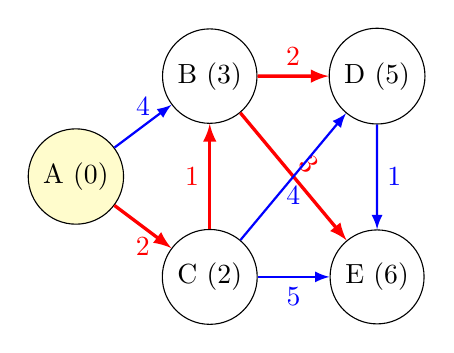
\begin{tikzpicture}[scale=0.85, auto, >=latex]
    \node[circle,draw,fill=yellow!20] (A) at (0,1.5) {A (0)};
    \node[circle,draw] (B) at (2,3) {B (3)};
    \node[circle,draw] (C) at (2,0) {C (2)};
    \node[circle,draw] (D) at (4.5,3) {D (5)};
    \node[circle,draw] (E) at (4.5,0) {E (6)};

    \draw[->,thick,blue] (A)-- node[above] {4} (B);
    \draw[->,very thick,red] (A)-- node[below] {2} (C);
    \draw[->,very thick,red] (C)-- node[left] {1} (B);
    \draw[->,very thick,red] (B)-- node[above] {2} (D);
    \draw[->,very thick,red] (B)-- node[above,sloped] {3} (E);
    \draw[->,thick,blue] (C)-- node[below] {4} (D);
    \draw[->,thick,blue] (C)-- node[below] {5} (E);
    \draw[->,thick,blue] (D)-- node[right] {1} (E);
\end{tikzpicture}
\caption{Dijkstra 算法执行示例与最终最短路径树（红色加粗边）}
\label{fig:dijkstra_trace}
\end{figure}

\subsection{另一种推导：贪心区域扩张}
从几何视角理解 Dijkstra 算法：维护一个已知最短距离的顶点集合 $R$（初始 $R = \{s\}$）。每次从 $V \setminus R$ 中选取距离 $s$ 最近的节点 $v$ 加入 $R$。由于所有边权均为正，$v$ 的最短路径上的前驱节点 $u$ 必定已经在 $R$ 中。因此寻找下一个加入 $R$ 的节点等价于在所有单边延伸路径中寻找最小值：
\[
\text{dist}(v) = \min_{u \in R, (u, v) \in E} \{\text{dist}(u) + l(u, v)\}.
\]

\subsection{运行时间与优先队列实现}

\begin{sidebarbox}{哪种堆（优先队列）最适合？ (Which heap is best?)}
Dijkstra 算法的运行时间高度依赖于底层优先队列的实现方式：
\begin{center}
\begin{tabular}{lccc}
\hline
实现方式 & \texttt{deletemin} & \texttt{insert/decreasekey} & 总时间复杂度 \\
\hline
无序数组 & $O(|V|)$ & $O(1)$ & $O(|V|^2)$ \\
二叉堆 & $O(\log |V|)$ & $O(\log |V|)$ & $O((|V| + |E|) \log |V|)$ \\
$d$ 叉堆 & $O(d \log_d |V|)$ & $O(\log_d |V|)$ & $O((|V| \cdot d + |E|) \frac{\log |V|}{\log d})$ \\
Fibonacci 堆 & $O(\log |V|)$ & $O(1)$ (摊还) & $O(|V| \log |V| + |E|)$ \\
\hline
\end{tabular}
\end{center}
对于稠密图（$|E| = \Theta(|V|^2)$），简单的数组实现即可达到 $O(|V|^2)$ 最优；对于稀疏图（$|E| = O(|V|)$），二叉堆表现极佳（$O(|V| \log |V|)$）；对于一般图，Fibonacci 堆理论性能最为优越。
\end{sidebarbox}

\section{存在负权边时的最短路径 (Shortest paths with negative edges)}

\subsection{负权边与松弛操作}
当图中存在负权边时，Dijkstra 算法的贪心选择性不再成立：通往某个节点的最短路径可能会经过距离更远的中间节点。
为了处理负权边，我们引入核心的\textbf{边松弛 (update / relax) 操作}：
\begin{algorithmic}[1]
\Procedure{update}{$(u, v) \in E$}
    \State $\text{dist}(v) = \min\{\text{dist}(v), \text{dist}(u) + l(u, v)\}$
\EndProcedure
\end{algorithmic}

任何不含负权环的最短路径最多包含 $|V| - 1$ 条边。如果我们将图中的所有边整体松弛 $|V| - 1$ 轮，那么无论最短路径的具体形态如何，其对应的边序列必然按顺序被松弛完毕。由此得到的 $O(|V| \cdot |E|)$ 算法就是著名的 \textbf{Bellman-Ford 算法}（图 4.13）。

\begin{figure}[htbp]
\centering
\begin{tcolorbox}[colback=white,colframe=gray!50!black,title={\textbf{图 4.13}\quad Bellman-Ford 算法}]
\begin{algorithmic}[1]
\Procedure{shortest-paths}{$G, l, s$}
    \State \textbf{Input:} 有向图 $G = (V, E)$，边权 $\{l_e\}$（无负权回路），起点 $s$
    \State \textbf{Output:} 从 $s$ 出发到各节点的最短距离 $\text{dist}(\cdot)$
    \For{所有 $u \in V$}
        \State $\text{dist}(u) = \infty,\; \text{prev}(u) = \text{nil}$
    \EndFor
    \State $\text{dist}(s) = 0$
    \State 重复 $|V| - 1$ 轮：
    \For{每一条边 $e \in E$}
        \State \Call{update}{$e$}
    \EndFor
\EndProcedure
\end{algorithmic}
\end{tcolorbox}
\label{fig:bellman_ford_alg}
\end{figure}

\subsection{负权回路检测 (Negative cycles)}
若图中包含总权重为负数的有向环路（负权回路），最短路径问题是病态无解的（绕环无限次可使路径长度趋于 $-\infty$）。
\textbf{检测机制}：在执行完 $|V| - 1$ 轮松弛后，额外再执行一轮全边松弛。若在第 $|V|$ 轮中依然存在某个顶点的 $\text{dist}$ 值被进一步减小，则图中必然存在负权回路。

\section{DAG 中的最短路径 (Shortest paths in dags)}

在有向无环图（DAG）中，由于不存在任何环路，负权回路的可能性被天然排除。在 DAG 中求解单源最短路径可以达到极致的\textbf{线性时间} $O(|V| + |E|)$！

\begin{property}
在 DAG 的任意路径上，顶点均按照拓扑排序的严格递增顺序出现。
\end{property}

算法流程：
\begin{enumerate}
    \item 使用 DFS 对 DAG 进行拓扑排序；
    \item 按照拓扑排序的先后顺序依次遍历每个顶点 $u$，并松弛从 $u$ 出发的所有出边 $(u, v) \in E$。
\end{enumerate}
该算法不要求边权非负，且通过将所有边权取反，可以直接在线性时间内求出 DAG 中的\textbf{最长路径}（在项目调度中对应关键路径 Critical Path 分析）。

\newpage
\section*{习题 (Exercises)}
\addcontentsline{toc}{section}{习题}

\begin{exercise}{4.1}
在给定带权图上从节点 $A$ 开始执行 Dijkstra 算法：(a) 给出每一步各节点的中间距离表；(b) 绘制最终的最短路径树。
\end{exercise}

\begin{exercise}{4.2}
在包含负权边的给定图上执行 Bellman-Ford 算法，列出每轮迭代后的距离向量。
\end{exercise}

\begin{exercise}{4.3}
设计运行时间不超过 $O(|V|^3)$ 的算法，检测无向图中是否存在长度恰为 4 的简单环。
\end{exercise}

\begin{exercise}{4.4}
分析利用 DFS 深度差寻找无向图最短环的错误提案并给出反例。
\end{exercise}

\begin{exercise}{4.5}
在单位权图上设计线性时间算法，计算从 $u$ 到 $v$ 的不同最短路径总数。
\end{exercise}

\begin{exercise}{4.6}
证明 Dijkstra 算法中的前驱指针数组 $\text{prev}$ 必定构成一棵树。
\end{exercise}

\begin{exercise}{4.7}
给定带权有向图 $G$ 和子图生成树 $T$，设计线性时间算法检验 $T$ 是否是以 $s$ 为起点的最短路径树。
\end{exercise}

\begin{exercise}{4.8}
分析“给所有边权加上一个巨大正数使其全为正后再运行 Dijkstra 算法”这一常见错误构想，并举出反例。
\end{exercise}

\begin{exercise}{4.9}
若有向图中仅有从起点 $s$ 出发的边权为负，其余边权均为正，Dijkstra 算法能否正确工作？证明你的结论。
\end{exercise}

\begin{exercise}{4.10}
若已知任意两点间的最短路径最多包含 $k$ 条边，给出在 $O(k|E|)$ 时间内求最短路径的算法。
\end{exercise}

\begin{exercise}{4.11}
在正权有向图中以 $O(|V|^3)$ 时间寻找全图最短有向环路。
\end{exercise}

\begin{exercise}{4.12}
在正权无向图中设计 $O(|V|^2)$ 算法寻找包含指定边 $e$ 的最短环。
\end{exercise}

\begin{exercise}{4.13}
汽车油箱容量约束下的可达性与最小油箱容量设计（瓶颈路径问题）。
\end{exercise}

\begin{exercise}{4.14}
在强连通有向图中设计算法，求解必须经过指定中间节点 $v_0$ 的全源最短路径对。
\end{exercise}

\begin{exercise}{4.15}
在 $O((|V| + |E|) \log |V|)$ 时间内判断从起点 $s$ 到各节点的最短路径是否唯一。
\end{exercise}

\begin{exercise}{4.16}
完全二叉堆与 $d$ 叉堆的数组存储索引换算，以及 $O(n)$ 建堆（\texttt{makeheap}）复杂度分析。
\end{exercise}

\begin{exercise}{4.17}
小整数边权 $[0, W]$ 下的 Dijkstra 算法加速：使用桶队列实现 $O(W|V| + |E|)$。
\end{exercise}

\begin{exercise}{4.18}
在费用相同的多条最短路径中，寻找经过中转次数（边数）最少的最短路径。
\end{exercise}

\begin{exercise}{4.19}
广义最短路径：同时包含边权延迟与路由器节点处理代价时的最短路径求解。
\end{exercise}

\begin{exercise}{4.20}
道路改建评估：在候选新路列表中选择一条加入网络，使得指定城市 $s$ 与 $t$ 之间的通行距离减少量最大。
\end{exercise}

\begin{exercise}{4.21}
\textbf{外汇套汇机会检测}：将汇率乘积套利转化为对数边权图上的负权回路检测问题。
\end{exercise}

\begin{exercise}{4.22}
\textbf{不定期货船问题 (Tramp steamer problem)}：使用二分搜索结合负权回路检测求解最大利润/成本比环路。
\end{exercise}
